\label{sec:model}
This section builds a simple toy model to understand how copyright might affect the reuse of digitized information.

\subsection*{Setup}

Consider a wikipedia page $W_{q,k}$ for an item of quality $q$ and knowledge level $k$. The quality is a parameter that captures how inherently interesting a topic is, for example a famous, well-known baseball player will have higher $q$ than a less well-known player. Knowledge level $k$ captures how much information exists on a given page. Let $q \in \{0,\infty\}$ and $k \in \{{1}/{4},\infty\}$.

Now define value, $V(W_{q,k})=\sqrt{q}+\sqrt{k}-\frac{k}{4}$ to be the value that the Wikipedia community delivers from a page $W_{q,k}$.  In a context like Wikipedia, $V$ could be the traffic that a page receives for example. Note that while $\frac{dV}{dq}>0$ and $\frac{dV}{dk}>0$, $\frac{d^2V}{dq^2}<0$ and $\frac{d^2V}{dk^2}<0$. This simply implies diminishing but positive marginal returns from increased information and increased player quality to $V$.

Define $C(W_{q,k})=\frac{k}{q}$ to be the cost of adding $k$ units of information to a page with quality level $q$. Here, $\frac{dC}{dk}>0$ implying higher costs of information acquistion for higher levels of knowledge, but $\frac{dC}{dq}<0$ , implying that it is easier to source information for higher quality topics, presumably because such information is more easily available. 

Under this setup, the Wikipedia community solves the following, simple maximization problem to determine optimal levels of $k$, i.e. $k^*$

$$k^* = \max_k \Big[ V(W_{q,k}) - C(W_{q,k}) \Big]$$

$$k^* = \max_k \Big[\sqrt{q}+\sqrt{k}-\frac{k}{4} - k/q\Big]$$

$$k^* = \frac{4q^2}{(q+4)^2}$$

\subsection*{Digitization and Copyright}

Now consider that a digitization project makes it easier to access information to a certain topic, but that these reduction in costs depend on the copyright status of the underlying material. For topics that can benefit from out-of-copyright material, this reduction in cost is greater than it is for in-copyright material. A general way to parameterize this change is to assume that costs of adding information are reduced differentially for different copyright status groups.

\newpage

Accordingly, let $$C_{in-copy}(W_{q,k})=\frac{C(W_{q,k})}{2}=\frac{k}{2q}$$ $$C_{out-of-copy}(W_{q,k})=\frac{C(W_{q,k})}{4}=\frac{k}{4q}$$

Solving a similar maximization problem as before, we now obtain:

$$k^*_{in-copy}= \frac{4q^2}{(q+2)^2}$$

$$k^*_{out-of-copy}= \frac{4q^2}{(q+1)^2}$$

Therefore, $k^*_{out-of-copy}>k^*_{in-copy}>k^*$. This setup delivers the first two results that we obtained in the main part of the paper, i.e. digitization increased amount of information for both in-copyright and out-of-copyright pages, but this increase is significantly greater for out-of-copyright pages. 

\subsection*{Differential Effects for Images vs. Text}

While the previous section modeled the idea that copyright restrictions create differential cost reductions for digital information, the differential impact of copyright by media type were not discussed. However, while it is possible to paraphrase textual material without violating copyright, reusing copyrighted images without violating copyright is harder.

Accordingly, let

$$C^{images}_{in-copy}(W_{q,k})=C^{text}_{in-copy}(W_{q,k})=\frac{C(W_{q,k})}{2}=\frac{k}{2q}$$

$$C^{images}_{out-of-copy}(W_{q,k})=\frac{C(W_{q,k})}{4}=\frac{k}{4q}$$
$$C^{text}_{out-of-copy}(W_{q,k})=\frac{C(W_{q,k})}{2}=\frac{k}{2q}$$

Solving the maximization problem, we obtain:

$$k^{*text}_{out-of-copy}=k^{*text}_{in-copy}= \frac{4q^2}{(q+2)^2}$$

$$k^{*images}_{out-of-copy}= \frac{4q^2}{(q+1)^2} \hspace{5mm} \Big >  \hspace{5mm} k^{*images}_{in-copy}= \frac{4q^2}{(q+2)^2}$$

Therefore, as is clear from this simple example, the differential cost reductions for images and text provides a direct prediction: the impact of copyright on reducing information reuse is driven primarily by a difference in the reuse of images rather than the reuse of textual information. 


\subsection*{Differential Effects by Quality Levels}

Now consider the impact of the copyright law on affecting increase in knowledge for topics of different quality types.

For in-copyright topics, percent increase in knowledge $\Delta k_{in-copy}=\frac{k^*_{in-copy}-k^*}{k^*}$ and similarly, for out-of-copyright topics, $\Delta k_{out-of-copy}=\frac{k^*_{out-of-copy}-k^*}{k^*}$. Solving we get:

$$ \Delta k_{in-copy} = \frac{4q^2}{(q+4)^2} \Big[ \frac{4(q+3)}{(q+2)^2} \Big] $$

$$ \Delta k_{out-of-copy} = \frac{4q^2}{(q+4)^2} \Big[ \frac{3(2q+5)}{(q+1)^2} \Big] $$

$$ \therefore \Delta = \Delta k_{out-of-copy} - \Delta k_{in-of-copy} = \frac{4q^2 (2q+3)}{(q+1)^2(q+2)^2} $$

%%\Big[\frac{(q+4)^2(2q+3)}{(q+1)^2(q+2)^2} \Big]$$

$$ \therefore \frac{d\Delta}{dk} = - \Big[ \frac{8q(q^3-6q-6)}{(q+1)^3(q+2)^3} \Big] $$

%%  \frac{2(q+4)(q^3+12q^2+30q+22)}{(q+1)^3(q+2)^3}   $$
%% \implies \boxed{\Delta > 0} \hspace{5mm} and

$$ \implies \hspace{5mm} \boxed{\frac{d\Delta}{dq} > 0 \hspace{5mm} \forall q \in (0, \approx 2.84)}  \hspace{5mm} and \hspace{5mm} \boxed{\frac{d\Delta}{dq} < 0 \hspace{5mm} \forall q \in (\approx 2.84,\infty)}$$

Therefore, under this simple model, while the increase in information reuse is greater for out-of-copyright topics than for in-copyright topics at the same quality level, this magnitude of this positive effect depends significantly on the quality level $q$ of the topic. For low $q$ (i.e. $0<q<\approx2.84$), higher quality topics experience a greater increase in information reuse as compared to lower quality topics. The intuition for this effect is simple, returns to information are higher for higher quality topics, and therefore a greater reduction in cost of adding information due to a lack of copyright is most beneficial for these topics. However, after a certain threshold, this logic no longer applies, and an increase in topic quality reduces the benefit from out-of-copyright status. The intuition for this effect is the following: higher quality topics had higher levels of initial information, and returns to adding more information are decreasing. Therefore, it becomes more valuable to add information to lower quality topics because these have a lower starting starting point, as compared to adding information to topics that already have higher levels of information to begin with.

In this way -- the model builds intuition for the key results of the paper, (i) digitization improves the quality of Wikipedia information, (ii) Copyright law reduces the potential benefits from digitiziation (iii) copyright mainly operates through the reuse of images rather than text and (iv) Potential benefits from a lack of copyright on digital material are greatest for topics of ``intermediate'' quality. 

\begin{center}
\textbf{Fig: A plot of how $\Delta$ varies with $q$}
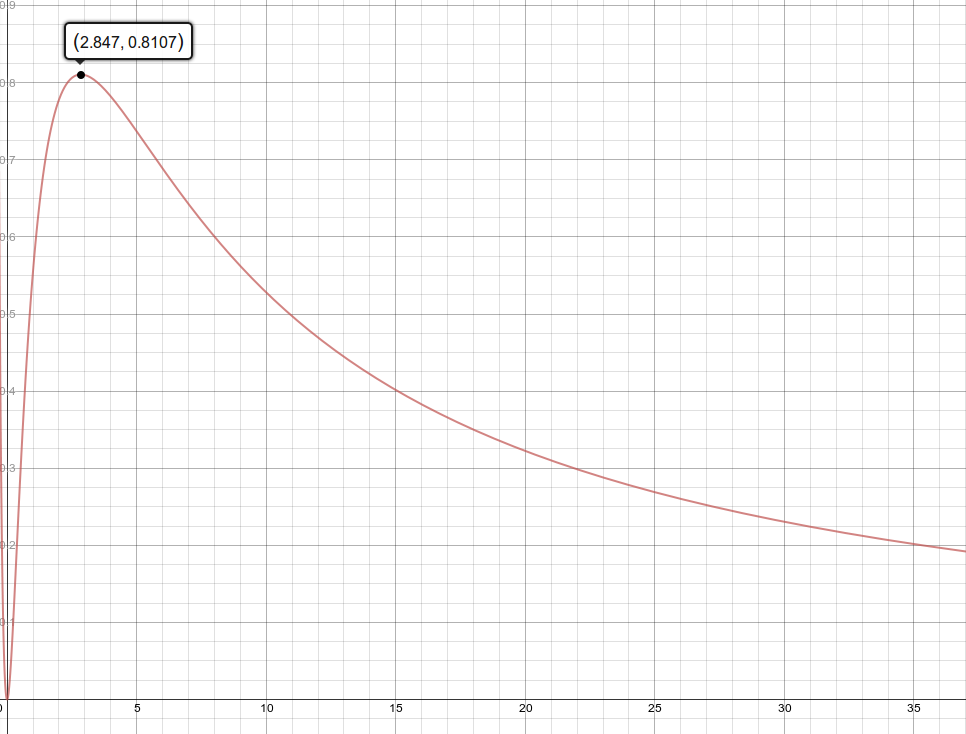
\includegraphics[scale = 0.3]{../tables/model.png}
\end{center}
  


%Now, for all $q \in \{0,\infy \}$, we have $\Delta k_{out-of-copy}>\Delta k_{in-copy}$







































